\section{Signaldarstellung im Frequenz- und Bildbereich}
\subsection{Fourierreihe periodischer Signale}
Die Überlagerung von Sinusschwingungen zu einem periodischen,
nichtsinusförmigen Signal nennt man harmonische Synthese.
\subsubsection{Reelle Fourierreihe}
\begin{mdframed}[style=exercise]
    \begin{itemize}
        \item mit $sin$ und $cos$:
            \[
                f(t) = a_0 \sum_{k=1}^\infty [a_k\cdot cos(k\omega_1 t) b_k\cdot sin(k\omega_1 t)]
            \]
        \item mit Amplitude und Phase:
            \begin{align*}
                f(t) &= A_0+\sum_{k=1}^\infty [A_k\cdot cos(k\omega_1 t + \varphi_k)]\\
                    &= A_0+\sum_{k=1}^\infty [A_k\cdot sin(k\omega_1 t + \varphi_k-\frac{\pi}{2})]
            \end{align*}

            \texttt{\footnotesize Koeffizienten }
            \[
                A_0 = \frac{1}{T}\int_{t_0}^{T+t_0} f(t)dt
            \]
            \begin{align*}
                a_k = \frac{2}{T}\int_{t_0}^{T+t_0} f(t)\cdot cos(k\omega_1 t) dt\\
                b_k = \frac{2}{T}\int_{t_0}^{T+t_0} f(t)\cdot sin(k\omega_1 t) dt
            \end{align*}
    \end{itemize}
\end{mdframed}

\subsubsection{Komplexe Fourierreihe}
\begin{mdframed}[style=exercise]
    \[
        f(t)=\sum_{k=-\infty}^{\infty} \underline{c}_k\cdot e^{j\omega_1 k t}
    \]
    \begin{align*}
        \underline{c}_k &= \frac{1}{T}\int_{t_0}^{T+t_0} f(t)\cdot e^{-j\omega_1 k t}dt
                        &= \frac{1}{2}\left( a_k-jb_k \right)
    \end{align*}
\end{mdframed}

\subsubsection{Komplex Reell umwandeln}
\begin{mdframed}[style=exercise]
    \begin{gather*}
    \texttt{\footnotesize Komplex $\rightarrow$ Reell:}\\
                a_0 = A_0 = \underline{c}_0\\
                \left.
                \begin{split}
                    a_k = 2\ \mathfrak{Re}\left\{ c_k \right\}= \left[ \underline{c}_k+\underline{c}_{-k} \right]\\
                    b_k = -2\ \mathfrak{Im}\left\{ \underline{c}_k \right\}= j\left[ \underline{c}_k-\underline{c}_{-k} \right]\\
                    A_k = 2|\underline{c}_k| \quad \beta_k = -\varphi_k
                \end{split}\right\} \quad k>0\\
    \texttt{\footnotesize Reell $\rightarrow$ Komplex:}\\
                \left.
                \begin{split}
                    \underline{c}_k = \frac{1}{2}\left( a_k-jb_k \right) = \frac{A_k}{2} e^{-j\beta_k}\\
                    \underline{c}_{-k} = \frac{1}{2}\left( a_k+jb_k \right) = \frac{A_k}{2} e^{j\beta_k}
                \end{split}\right\} \quad k>0\\
    \end{gather*}
\end{mdframed}

\subsubsection{Symmetrieeigenschaften}
\begin{itemize}
    \item Gerade Funktionen
        symmetrisch zur y-Achse\\
        alle $sin$-teile verschwinden
        - $A_0 = \frac{2}{T}\int^{\frac{T}{2}}_{0} y(t)dt$\\
        - $a_{k} = \frac{4}{T}\int^{\frac{T}{2}}_{0}y(t)\cdot cos(k\omega_1t)dt$\\
        - $b_k = 0$\\
    \item Ungerade Funktionen
        symmetrisch zum Ursprung\\
        alle $cos$-teile und Gleichanteil verschwinden

        - $A_0 = 0$\\
        - $a_k = 0$\\
        - $b_{k} = \frac{4}{T}\int^{\frac{T}{2}}_{0} y(t)\cdot sin(k\omega_1t)dt$\\
\end{itemize}
\subsubsection{Halbwellensymmetrie}
Halbwellensymmetrie gilt wenn:
\[
    y(t) = -y(t \pm T/2)
\]
Die Fourier-Reihe einer Zeitfunktion mit HWS enthält stets
nur Terme mit ungeraden Ordnungszahlen. $k=1,3,5,\dots,\infty$
\begin{mdframed}[style=exercise,frametitle=im Allgemeinen]
    \texttt{\footnotesize Koeffizienten}:\\
    \[
        A_0 = 0,\
        a_{2k} = 0,\
        b_{2k} = 0
    \]
        $$a_{2k-1} = \frac{4}{T}\int^{\frac{T}{2}}_{0}y(t)\cdot cos((2k-1)\omega_1t)dt$$
        $$b_{2k-1} = \frac{4}{T}\int^{\frac{T}{2}}_{0}y(t)\cdot sin((2k-1)\omega_1t)dt$$
\end{mdframed}
\begin{mdframed}[style=exercise,frametitle=gerade Halbwellensymmetrie]
    \[
        A_0 = 0,\
        b_k = 0,\
        a_{2k} = 0
    \]
    $$a_{2k-1} = \frac{8}{T}\int^{\frac{T}{4}}_{0}y(t)\cdot cos((2k-1)\omega_1t)dt$$
\end{mdframed}
\begin{mdframed}[style=exercise,frametitle=ungerade Halbwellensymmetrie]
    \[
        A_0 = 0,\
        a_k = 0,\
        b_{2k} = 0
    \]
    $$b_{2k-1} = \frac{8}{T}\int^{\frac{T}{4}}_{0}y(t)\cdot sin((2k-1)\omega_1t)dt$$
\end{mdframed}

\subsubsection{Verschiebungssatz}
Verschiebung im Zeitbereich entspricht eine Drehung den Komplexen Spektrum um
die Phase $\rightarrow\ -k\omega_1 t_v$
\begin{align*}
    f_v(t) = f(t-t_v) &= \sum_{k=-\infty}^{\infty} \underline{c}_k\cdot e^{j\omega_1 k (t-t_v)} \\
           &= \sum_{k=-\infty}^{\infty} \underbrace{\underline{c}_k\cdot e^{j\omega_1 k t_v}}_{\underline{c}_{k_v}} \cdot e^{\omega_1 k t}
\end{align*}

Ist tv < 0, wie im Beispiel oben, so werden die Phasenwinkel des Spektrums mit
zunehmender Frequenz größer.

\subsubsection{Fourierreihe und LTI-Systeme}

\[
    y(t) = \sum_{k=-\infty}^{\infty} \underbrace{\underline{H}(k\omega_1)\cdot\underline{c}_{xk}}_{\underline{c}_{yk}} \cdot e^{j\omega_1 k t}
\]

\subsection{Kenngrößen periodischer Signale}
\begin{itemize}
    \item Effektivwert
        \[
            \boxed{U_{\mathit{eff}} = \sqrt{\frac{1}{T} \int_\tau^{\tau+T} u(t)^2 dt}}
        \]
    \begin{mdframed}[style=exercise]
        mit der Fourierreihe:
        $$ U_{\mathit{eff}} = \sqrt{\sum_{k=-\infty}^{\infty} c_k^2} = \sqrt{\sum_{k=-\infty}^{\infty}U_{k,\mathit{eff}}^2} $$
        auch:
        $$ \sqrt{A_0^2 + \frac{1}{2} \sum_{k=1}^{\infty} A_k^2} $$
    \end{mdframed}
    \item Klirrfaktor(Oberschwingungsgehalt):\\
        Dient zur Quantifizierung einer nichtlinearen Verzerrung bzw. von der
        Sinusform eines Signals.
        \begin{align*}
            k &= \frac{\text{Effektivwert der Oberschwingungen}}{\text{Effektivwert des Wechselanteil}} \\
            &= \boxed{\frac{\sqrt{\sum_{{\color{red}{k=2}}}^{\infty} U_{k}^{2}}}{\sqrt{\sum_{\color{red}{k=1}}^{\infty} U_{k}^{2}}} = \frac{\sqrt{U_\sim^2 - U_1^2}}{U_\sim} \leq 1}
        \end{align*}
        Für Wechselgrößen lässt sich $k$ einfach mit \textbf{Grundschwingungsgehalt} $g$ ermitteln (\textit{gilt immer}):
        \[
            \boxed{k = \sqrt{1-g^2} \leftrightarrow g = \frac{U_1}{U}}
        \]
    \item Mischgrößen\\
        - Schwingungsgehalt:
        \[
            s = \frac{U_\sim}{U} = \frac{\textsc{Effektivwert des Wechselanteils}}{\textsc{Effektivwert der Mischgröße}}
        \]
        - Welligkeit:
        \[
            w = \frac{U_\sim}{\bar{U}} = \frac{\textsc{Effektivwert des Wechselanteils}}{\textsc{Gleichanteil}}
        \]
        - Riffelfaktor:
        \[
            R = \frac{\hat{U}_\sim}{\bar{U}} = \frac{\textsc{Scheitelwert des Wechselanteils}}{\textsc{Gleichanteil}}
        \]
    \item Wirkleistung:
        \[
            P = \bar{p}(t) = \frac{1}{T} \int_0^T u(t)\cdot i(t) dt
        \]
        \[
            P = \sum_{k=-\infty}^{\infty}\underline{u}_k \underline{i}_k^* \leftrightarrow i_k^* = i_{-k}
        \]
        \begin{mdframed}[style=exercise]
            Als Reihe:
            \[
                P_0 + \sum_{k=1}^{\infty} U_{k_{eff}}\cdot
                I_{k_{eff}}\cdot\cos(\varphi_{uk}-\varphi_{ik}) = \sum_{k=0}^{\infty}P_k
            \]
        \end{mdframed}
        Nur gleichfrequente harmonische tragen zur Wirkleistung bei!
    \item Schein- und Blindleistung\\
        \[
            \boxed{S = U_{eff}\cdot I_{eff} = U\cdot I = \sqrt{P^2+Q^2}}
        \]
        \begin{mdframed}[style=exercise]
        Bei einem nicht linearen Verbraucher an einer Sinusförmigen Spannung:
        \vspace{-1em}
            \begin{multline*}
                S^{2}=(U I)^{2}=U_{1}^{2} \cdot \sum_{k=0}^{\infty} I_{k}^{2}=\\U_{1}^{2} I_{0}^{2}+U_{1}^{2} \sum_{k=2}^{\infty} I_{k}^{2}+U_{1}^{2} I_{1}^{2} \sin ^{2} \varphi_{1}+U_{1}^{2} I_{1}^{2} \cos ^{2} \varphi_{1}
            \end{multline*}
        \end{mdframed}

        Räumlich Darstellung der Scheinleistung:
        \begin{center}
            \vspace{-1em}
            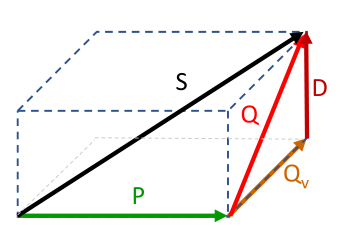
\includegraphics[width=0.35\columnwidth]{Schein-Blindleistung_raeumlich.png}
            \vspace{-0.7em}
        \end{center}

        \begin{mdframed}[style=exercise,frametitle=Verschiebungs- Feldblindleistung $Q_v$]
            \vspace{-1em}
            \begin{gather*}
                Q = \sqrt{Q^2_v + D^2}\\
                S = \sqrt{P^2+Q^2_v + D^2}
            \end{gather*}
            Blindleistung aufgrund der Phasenverschiebung zwischen Strom und
            Spannung gleicher Frequenz.
        \end{mdframed}
        \begin{mdframed}[style=exercise,frametitle=Verzerrungblindleistun $D$]
            \[
                D^2 = U_1^2\cdot(I^2-I_1^2) = S^2(1-g)
            \]
            von Mischtermen (Produkten von Spannung und Strom unterschiedlicher
            Frequenzen).
        \end{mdframed}
\end{itemize}

\subsection{Fouriertransformation}
\begin{mdframed}[style=exercise]
    \[
        x(t) \laplace X(\omega)
    \]
    Hintransformation - Analysegleichung:
    \[
        \underline{X}(\omega)=\mathcal{F}\left\{ x(t) \right\} = \int_{-\infty}^{\infty} x(t) \cdot e^{-j\omega t} dt
    \]
    Komplexwertige Fouriertransformierte:
    \[
        \underline{X}(\omega) = |\underline{X}(\omega)|\cdot e^{j\omega\varphi}
    \]
    \footnotesize
    $$\textsc{Einheit:} \left[ x(t) \right]\cdot s$$

    \normalsize

    Rücktransformation - Synthesegleichung:
    \[
        x(t) = \mathcal{F}^{-1}\left\{ \underline{X}(\omega) \right\} = \frac{1}{2\pi}\int_{-\infty}^{\infty} \underline{X}(\omega) \cdot e^{j\omega t} d\omega
    \]
\end{mdframed}

\subsubsection{Umwandeln zwischen Fouriertransformation und Fourierreihen}
$\text{Grenzübergang\ }
    T\rightarrow\infty$
\[
    \omega_1=\frac{2\pi}{T}\rightarrow0\ \rightarrow
    \text{kontinuierliches Spektrum}
\]

\[
    \boxed{ \text{FR}\rightarrow\text{FT: }\quad \underline{c}_k =
    \frac{1}{T}\underline{X}(\omega_1)}
\]

\[
    \boxed{ \text{FR}\rightarrow\text{FT: }\quad \underline{X}(\omega) =
    2\pi\sum_{k=-\infty}^{\infty} \underline{c}_k\cdot
    \delta(\omega-k\omega_1)}
\]

\subsection{Eigenschaften der Fouriertransformation}
\begin{mdframed}[style=exercise,frametitle=Symmetrie,nobreak=false]
            \begin{wrapfigure}[10]{R}{0.27\textwidth}
                \vspace{-1.4em}
                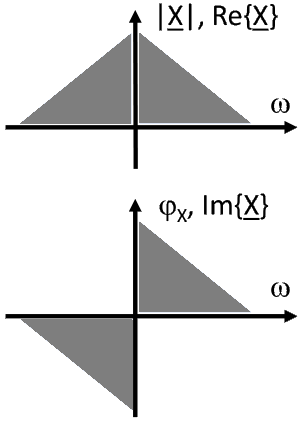
\includegraphics[width=0.3\textwidth]{FT_Symmetrie.png}
            \end{wrapfigure}

           \begin{minipage}{5cm}
                Betrag und der Realteil des Spektrums sind gerade\\
            \end{minipage}

            \begin{minipage}{5cm}
                Phase und der Imaginärteil des Spektrums sind ungerade.
            \end{minipage}

            \[
                \underline{X}(-\omega) = \underline{X}^*(\omega)
            \]
            % \begin{itemize}
            %     \footnotesize
            %     \item Betrag und der Realteil des Spektrums sind gerade

            %     \item Phase und der Imaginärteil des Spektrums sind ungerade.
            % \end{itemize}

            \begin{gather*}
                x(t)\text{ reel und gerade}\rightarrow X(\omega)\text{ reel und gerade}\\
                \underline{X}(\omega) = 2\int_0^\infty x(t)\cos(\omega t)dt\\
                x(t)\text{ reel und ungerade}\rightarrow X(\omega)\text{ imaginär und ungerade}\\
                \underline{X}(\omega) = -2j\int_0^\infty x(t)\sin(\omega t)dt
            \end{gather*}
\end{mdframed}
\begin{mdframed}[style=exercise,nobreak=false]
\begin{itemize}
    \item \textbf{Linearität}
        \[
            a_{1} x_{1}(t)+a_{2} x_{2}(t)\ \laplace\  a_{1} \underline{X}_{1}(\omega)+a_{2} \underline{X}_{2}(\omega)
        \]
        % {\footnotesize Eine lineare Überlagerung von gewichteten Zeitsignalen führt zur linearen
        % Überlagerung der Spektren mit denselben Vorfaktoren.}
    \item \textbf{Dualität}
        \[
            \underline{X}(t)\ \laplace\  2\pi\cdot x(-\omega)
        \]
        % {\footnotesize Zeit- und Frequenzbereich können vertauscht werden (bis auf den Faktor $2\pi$
        % und einer Vorzeichenumkehr).}
    \item \textbf{Zeitskalierung}
        \[
            x(a \cdot t)\ \laplace\ \frac{1}{|a|} \underline{X}\left(\frac{\omega}{a}\right) \quad a \in \mathbb{R} \backslash\{0\}
        \]
        % {\footnotesize Eine Stauchung der Zeitachse führt zur Dehnung der Frequenzachse.
        % Frequenzachse (und Skalierung der Amplitude).}
    \item \textbf{Frequenzskalierung}
        \[
            \frac{1}{|b|} x\left(\frac{t}{b}\right)\ \laplace\ \underline{X}(b\cdot\omega) \quad b \in \mathbb{R} \backslash\{0\}
        \]
        % {\footnotesize Eine Stauchung der Frequenzachse führt zur Dehnung der Zeitachse.
        % Zeitachse (und Skalierung der Amplitude).}
    \item \textbf{Zeitverschiebung}
        \[
            x\left(t-t_{0}\right)\ \laplace\ \underline{X}(\omega) \cdot e^{-j \omega t_{0}}
        \]
        % {\footnotesize Eine Verschiebung im Zeitbereich ändert nicht den Betrag des Spektrums,
        % aber die Phase um einen sich mit der Frequenz $\omega$ linear ändernden Phasenterm.}
    \item \textbf{Frequenzverschiebung - Modulation}
        \[
            x(t) \cdot e^{j \omega_{0} t}\ \laplace\ \underline{X}\left(\omega-\omega_{0}\right)
        \]
        % {\footnotesize Eine Verschiebung im Frequenzbereich führt zu einem Modulationsterm im
        % Zeitbereich oder andersherum, um eine Frequenzverschiebung zu erreichen,
        % muss im Zeitbereich mit $e^{(j\omega_0t)}$ multipliziert (moduliert) werden.}
    \item \textbf{Faltungssatz}
        \[
            x_{1}(t) * x_{2}(t)\ \laplace\ \underline{X}_{1}(\omega) \cdot \underline{X}_{2}(\omega)
        \]
        % {\footnotesize Faltung im Zeitbereich entspricht Multiplikation im Frequenzbereich}
    \item \textbf{Multiplikation - Fenstertheorem}
        \[
            x_{1}(t) \cdot x_{2}(t)\ \laplace\ \frac{1}{2 \pi} \underline{X}_{1}(\omega) * \underline{X}_{2}(\omega)
        \]
        % {\footnotesize Multiplikation im Zeitbereich entspricht Faltung im Frequenzbereich (und
        % Normierung mit $2\pi$).}
    \item \textbf{Differentiation\\}
        {\small im Zeitbereich:}
        \[
            \frac{d}{dt} x(t) \ \laplace\ j\omega\underline{X}(\omega)
        \]
        {\small im Frequenzbereich:}
        \[
            t \cdot x(t)\ \laplace\ j \frac{d}{d \omega} \underline{X}(\omega)
        \]
        % {\footnotesize Differenzieren im Zeitbereich dreht die Phase des Spektrums um $\frac{\pi}{2}$ und
        % verstärkt die Amplitude des Spektrums zu hohen Frequenzen hin mit linear
        % anwachsendem $\omega$.}
    \item \textbf{Integration}
        \[
            \int_{-\infty}^{t} x(\tau) d \tau\ \laplace\ \frac{1}{j \omega} \underline{X}(\omega)+\pi \cdot \underline{X}(0) \cdot \delta(\omega)
        \]
        % {\footnotesize Integrieren dreht die Phase um $-\frac{\pi}{2}$, dämpft die Amplitude des
        % Spektrums mit $\frac{1}{\omega}$ und erzeugt einen (dem Gleichanteil von
        % $x(t)$ entsprechenden) Dirac bei $\omega = 0$.}
    \item \textbf{Energieberechnung - Parseval}
        \[
            \int_{-\infty}^{+\infty}|x(t)|^{2} d t=\frac{1}{2 \pi} \int_{-\infty}^{+\infty}|\underline{X}(\omega)|^{2} d \omega
        \]
        % {\footnotesize Die Signalenergie lässt sich aus der Zeit- und Frequenzbereichsdarstellung berechnen.}
\end{itemize}
\end{mdframed}
